\documentclass[12pt]{article}
\usepackage[left=1cm, right=1cm, top=2cm,bottom=1.5cm]{geometry} 

\usepackage[parfill]{parskip}
\usepackage[utf8]{inputenc}
\usepackage[T2A]{fontenc}
\usepackage[russian]{babel}
\usepackage{enumitem}
\usepackage[normalem]{ulem}
\usepackage{amsfonts, amsmath, amsthm, amssymb, mathtools}
\usepackage{tikz}
\usepackage{tabularx}
\usepackage{hhline}

\usepackage{accents}
\usepackage{fancyhdr}
\pagestyle{fancy}
\renewcommand{\headrulewidth}{1.5pt}
\renewcommand{\footrulewidth}{1pt}

\usepackage{graphicx}
\usepackage[figurename=Рис.]{caption}
\usepackage{subcaption}
\usepackage{float}

%%Наименование папки откуда забирать изображения
\graphicspath{ {./images/} }

%%Изменение формата для ввода доказательства
\renewcommand{\proofname}{$\square$  \nopunct}
\renewcommand\qedsymbol{$\blacksquare$}

%%Изменение отступа на таблицах
\addto\captionsrussian{%
	\renewcommand{\proofname}{$\square$ \nopunct}%
}
%% Римские цифры
\newcommand{\RN}[1]{%
	\textup{\uppercase\expandafter{\romannumeral#1}}%
}

%% Для удобства записи
\newcommand{\MR}{\mathbb{R}}
\newcommand{\MQ}{\mathbb{Q}}
\newcommand{\MC}{\mathbb{C}}
\newcommand{\MK}{\mathbb{K}}
\newcommand{\MI}{\mathrm{I}}
\newcommand{\MJ}{\mathrm{J}}
\newcommand{\MH}{\mathrm{H}}
\newcommand{\MT}{\mathrm{T}}
\newcommand{\MU}{\mathcal{U}}
\newcommand{\MV}{\mathcal{V}}
\newcommand{\VN}{\varnothing}
\newcommand{\VE}{\varepsilon}
\newcommand{\id}{\mathrm{id}}
\newcommand{\Mat}{\text{Mat}}
\newcommand{\RE}{\operatorname{Re}}
\newcommand{\IM}{\operatorname{Im}}

\theoremstyle{definition}
\newtheorem{defn}{Опр:}
\newtheorem{rem}{Rm:}
\newtheorem{prop}{Утв.}
\newtheorem{exrc}{Упр.}
\newtheorem{lemma}{Лемма}
\newtheorem{theorem}{Теорема}
\newtheorem{corollary}{Следствие}

\newenvironment{cusdefn}[1]
{\renewcommand\thedefn{#1}\defn}
{\enddefn}

\DeclareRobustCommand{\divby}{%
	\mathrel{\text{\vbox{\baselineskip.65ex\lineskiplimit0pt\hbox{.}\hbox{.}\hbox{.}}}}%
}
%Короткий минус
\DeclareMathSymbol{\SMN}{\mathbin}{AMSa}{"39}
%Длинная шапка
\newcommand{\overbar}[1]{\mkern 1.5mu\overline{\mkern-1.5mu#1\mkern-1.5mu}\mkern 1.5mu}
%Функция знака
\DeclareMathOperator{\sgn}{sgn}

%Операторы ядра и образа
\DeclareMathOperator{\Ker}{Ker}
\DeclareMathOperator{\Ima}{Im}
\DeclareMathOperator{\tr}{tr}


%% Шапка для букв сверху
\newcommand{\wte}[1]{\widetilde{#1}}

%Обозначение константы
\DeclareMathOperator{\const}{\text{const}}

%Интеграл в большом формате
\DeclareMathOperator{\dint}{\displaystyle\int}
\newcommand{\ddint}[2]{\displaystyle\int\limits_{#1}^{#2}}


\newcommand{\smallerrel}[1]{\mathrel{\mathpalette\smallerrelaux{#1}}}
\newcommand{\smallerrelaux}[2]{\raisebox{.1ex}{\scalebox{.75}{$#1#2$}}}

\newcommand{\smallin}{\smallerrel{\in}}
\newcommand{\smallnotin}{\smallerrel{\notin}}

\newcommand*{\medcap}{\mathbin{\scalebox{1.25}{\ensuremath{\cap}}}}%
\newcommand*{\medcup}{\mathbin{\scalebox{1.25}{\ensuremath{\cup}}}}%

%Скалярное произведение
\DeclarePairedDelimiterX{\inner}[2]{\langle}{\rangle}{#1, #2}

%Подпись символов снизу
\newcommand{\ubar}[1]{\underaccent{\bar}{#1}}

\newcommand*\circled[1]{\tikz[baseline=(char.base)]{
		\node[shape=circle,draw,inner sep=2pt] (char) {#1};}}


\begin{document}
\lhead{Линейная алгебра}
\chead{Мануйлов В.М.}
\rhead{Лекция - 7}
\section*{Ортогональные проекции}
Пусть $L \subset V, \, a \in V$, тогда $a = a_1 + a_2$, где $a_1 \in L, \, a_2 \in L^\bot$. 

\begin{defn}
	\uwave{Ортогональной проекцией} $a \in V$ назовем $a_1 \in L$, обозначение $a_{\|}$.
\end{defn}
\begin{defn}
	\uwave{Ортогональной составляющей} $a \in V$ назовем $a_2 \in L^\bot$, обозначение $a_\bot$.
\end{defn}
Любой вектор можно представить в виде ортогональной проекции и ортогональной составляющей: 
$$
	L \subset V, \,\forall  a \in V, \, \exists! \, a = a_{\|} + a_\bot, \, a_{\|} \in L, \, a_\bot \in L^\bot
$$

\subsection*{Расстояние от вектора до подпространства $L$}
\begin{lemma}
	Запишем один и тот же вектор двумя способами: $a \in V \Rightarrow a = a_{\|} + a_\bot = a_1 + a_2$, где $a_1 \in L$. Тогда верно следующее неравенство: 
	$$
		|a_\bot| \leq |a_2|
	$$
\end{lemma}
\begin{figure}[H]
	\centering
	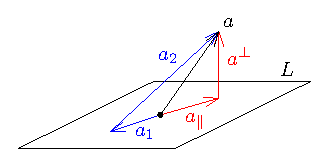
\includegraphics[width=0.35\textwidth]{7_1.eps}
	\label{7_1}
	\caption{Расстояние от $a$ до $L$.}
	\label{fig:Расстояние от $a$ до $L$}
\end{figure}
\begin{proof}
	Заметим, что $|a_\bot|^2 = |a - a_{\|}|^2 = (a - a_{\|}, a - a_{\|})$, а также $\forall a \in L, \, (a, a_\bot) = 0$. Тогда:
	$$
		a_1, a_{\|} \in L \Rightarrow (a_1, a_\bot) = (a_{\|}, a_\bot) = 0
	$$
	Рассмотрим длину вектора $a_2$:
	$$
		|a_2|^2 = |a - a_1|^2 = |a_{\|} + a_\bot - a_1|^2 = (a_{\|} + a_\bot - a_1,a_{\|} + a_\bot - a_1 ) = 
	$$
	$$
		=	(a_{\|}, a_{\|} + a_\bot - a_1) + (a_\bot, a_{\|} + a_\bot - a_1) - (a_1, a_{\|} + a_\bot - a_1) = 
	$$
	$$
		=(a_{\|}, a_{\|}) + (a_{\|}, a_{\bot}) - (a_{\|},a_1) + (a_{\bot}, a_{\|}) + (a_{\bot}, a_{\bot}) - (a_{\bot},a_1) - (a_1, a_{\|}) - (a_1, a_{\bot}) + (a_1,a_1) =
	$$
	$$
		 = (a_{\|},a_{\|}) + (a_\bot, a_\bot) + (a_1,a_1) - 2(a_{\|},a_1) = |a_\bot|^2 + (a_{\|},a_{\|} - a_1) + (a_1, a_1 - a_{\|}) =
	$$
	$$
		= |a_\bot|^2 + (a_{\|},a_{\|} - a_1) + (- a_1, a_{\|} - a_1)= |a_\bot|^2 + \underbrace{(a_{\|} - a_1, a_{\|} - a_1)}_{\geq 0} \geq |a_\bot|^2
	$$
	где последнее неравенство верно в силу свойств скалярного произведения.
\end{proof}
\begin{defn}
	\uwave{Расстояние от} $a \in V$ \uwave{до} $L$ это длина ортогональной проекции $|a_\bot|$.
\end{defn}
\begin{lemma}
	Угол $(\widehat{a,a_{\|}})$ не больше, чем угол $(\widehat{a,a_1})$, при условии, что $a_1 \neq 0$. Или по другому:
	$$
		(\widehat{a,a_{\|}}) \leq (\widehat{a,a_1}), \, a_1 \neq 0, \, a_1 \in L
	$$
	где косинус угла между векторами мы понимаем в стандартном смысле: $\cos({\widehat{a,b}}) = \dfrac{(a,b)}{|a|{\cdot}|b|}$.
\end{lemma}
\begin{proof}
	Пусть $a = a_1 + a_2 = b_1 + b_2$, где $a_1 \bot a_2, \, b_1 \bot b_2$. Тогда, если $|b_1| \geq |a_1|$, то: 
	$$
		(\widehat{a,a_1}) \geq (\widehat{a,b_1}) \Leftrightarrow \cos(\widehat{a,a_1}) \leq \cos(\widehat{a,b_1}), \, \sin(\widehat{a,a_1}) \geq \sin(\widehat{a,b_1})
	$$
	Или по-другому это можно записать следующим образом:
	$$
		\cos(\widehat{a,a_1}) = \dfrac{(a,a_1)}{|a|{\cdot}|a_1|} \leq \dfrac{(a,b_1)}{|a|{\cdot}|b_1|} = \cos(\widehat{a,b_1}) \Leftrightarrow \dfrac{(a_1, a_1)}{|a|{\cdot}|a_1|} = \dfrac{|a_1|}{|a|} \leq \dfrac{(b_1,b_1)}{|a|{\cdot}|b_1|} = \dfrac{|b_1|}{|a|} \Leftrightarrow |a_1| \leq |b_1|
	$$
	Рассмотрим скалярное произведение вектора $a$ с самим собой:
	$$
		(a,a) = (a_1,a_1) + (a_1,a_2) + (a_2,a_1) + (a_2, a_2) = (a_1, a_1) + (a_2, a_2) \Leftrightarrow |a|^2 = |a_1|^2 + |a_2|^2 = |b_1|^2 + |b_2|^2
	$$
	Следовательно, если $|b_1| \geq |a_1|$, то $|b_2| \leq |a_2|$ и $(\widehat{a,a_1}) \geq (\widehat{a,b_1})$. 
	
	Заменим теперь $a_1$ на $a_1^\prime =  \lambda a_1$ и подберем $\lambda$ таким образом, чтобы $\lambda a_1 \bot a_2^\prime$, где $a_2^\prime = a - \lambda a_1, \, a = a_1^\prime + a_2^\prime$. Таким образом:
	$$
		\lambda a_1 \bot a_2^\prime \Leftrightarrow (\lambda a_1, a - \lambda a_1) = 0 \Rightarrow \lambda (a_1, a - \lambda a_1) = 0
	$$
	Поскольку $a_1 \neq 0$ по условию и случай $\lambda = 0$ нас не интересует, то $\lambda \neq 0$ и верно следующее: 
	$$	
		(a_1,a) - \lambda (a_1,a_1) = 0 \Rightarrow \lambda = \dfrac{(a_1,a)}{(a_1,a_1)}, \, a_1 \neq 0 \Rightarrow (a_1,a_1) \neq 0
	$$
	Рассмотрим угол между $a$ и $a_1$ и угол между $a$ и $\lambda a_1$: 
	$$
		\lambda > 0 \Rightarrow (\widehat{a,a_1}) = (\widehat{a,a_1^\prime}), \, \lambda < 0 \Rightarrow (\widehat{a,a_1}) = \pi - (\widehat{a,a_1^\prime})
	$$
	Знак $\lambda$ определяется слагаемым $(a_1,a)$: если $(\widehat{a,a_1}) \leq \dfrac{\pi}{2} \Rightarrow \lambda > 0$, если $(\widehat{a,a_1}) \geq \dfrac{\pi}{2} \Rightarrow \lambda < 0$. Это видно, если смотреть на формулу косинуса угла между векторами: 
	$$
		(\widehat{a,a_1}) \geq \dfrac{\pi}{2} \Rightarrow \cos(\widehat{a,a_1}) < 0 \Rightarrow \dfrac{(a,a_1)}{|a|{\cdot}|a_1|} < 0 \Rightarrow (a,a_1) = (a_1,a) < 0 \Rightarrow \lambda = \dfrac{(a_1,a)}{(a_1,a_1)} < 0
	$$
	Заметим также, что угол между вектором и его проекцией всегда острый $\Rightarrow (\widehat{a,a_{\|}}) \leq \dfrac{\pi}{2}$, поэтому если $(\widehat{a,a_1}) \geq \dfrac{\pi}{2}$, то требуемое - очевидно. Рассмотрим случай $(\widehat{a,a_1}) \leq \dfrac{\pi}{2}, \, \lambda >0$, тогда $(\widehat{a,a_1}) = (\widehat{a,a_1^\prime})$. По предыдущей лемме: $|a_\bot| \leq |a_2^\prime|$.
	\begin{figure}[H]
		\centering
		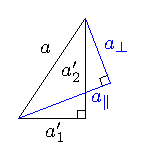
\includegraphics[width=0.11\textwidth]{7_2.eps}
		\label{7_2}
		\caption{Длина $a_\bot$ и $a_2^\prime$.}
		\label{fig:Расстояние от $a$ до $L$}
	\end{figure}
	Тогда верно следующее:
	$$
		|a|^2 = |a_\bot|^2 + |a_{\|}|^2 = |a_1^\prime|^2 + |a_2^\prime|^2 \Rightarrow |a_{\|}| \geq |a_1^\prime| \Rightarrow (\widehat{a,a_{\|}}) \leq (\widehat{a,a_1^\prime})
	$$
	поскольку напротив большей стороны лежит больший угол. Так как $\lambda >0$, то:
	$$
		(\widehat{a,a_{\|}}) \leq (\widehat{a,a_1^\prime}) = (\widehat{a,a_1}) \leq \dfrac{\pi}{2}
	$$
\end{proof}
\begin{defn}
	\uwave{Углом между вектором и подпространством} называется угол между вектором и его проекцией. При этом этот угол - наименьший, то есть $(\widehat{a,a_{\|}})$.
\end{defn}
\newpage
\section*{Матрица Грама}
Пусть $a_1, \dotsc, a_n$ - набор векторов.
\begin{defn}
	\uwave{Матрицей Грама} из набора векторов $a_1, \dotsc, a_n$ называется матрица: 
	$$
		G = G(a_1, \dotsc, a_n) = 
		\begin{pmatrix}
			(a_1,a_1) & \dotsc & (a_1, a_n) \\
			\vdots & \ddots & \vdots \\
			(a_n, a_1) & \dotsc & (a_n, a_n)
		\end{pmatrix}
	$$
	составленная из скалярных произведений $(a_i, a_j)$.
\end{defn}
\subsection*{Объем параллелепипедов}
\begin{defn}
	\uwave{Параллелепипед}, построенный по векторам $a_1, \dotsc, a_n$ есть следующее множество:
	$$
		P(a_1, \dotsc, a_n) = \{t_1 a_1 + \dotsc + t_n a_n \colon 0 \leq t_i \leq 1\}
	$$
\end{defn}
Например, рассмотрим параллелепипед построенный на векторах $a_1, a_2$:
\begin{figure}[H]
	\centering
	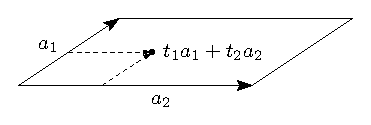
\includegraphics[width=0.4\textwidth]{7_3.eps}
	\label{7_3}
	\caption{Задание точек параллелепипеда $P(a_1,a_2)$.}
	\label{fig:Задание точек параллелепипеда}
\end{figure}
Все точки на нём можно задать через $P(a_1,a_2) = \{t_1 a_1 + t_2 a_2 \colon 0 \leq t_i \leq 1\}$.

Пусть $V_n$ это $n$-мерный объем $P(a_1, \dotsc, a_n)$. Определеим $V_n$ по индукции:
\begin{enumerate}[label ={(\arabic*)}]
	\item $n=1 \Rightarrow P(a_1) = \{t_1 a_1 \colon t_1 \in [0,1]\} \Rightarrow V_1(P(a_1)) \coloneqq|a_1|$;
	\item $n=2 \Rightarrow V_2(P(a_1,a_2)) \coloneqq |a_1|{\cdot}d(a_2,\langle a_1 \rangle)$, то есть произведение основания на высоту, где мы обозначили $d(a,L)$ - \uwave{расстояние от вектора $a$ до $L$};
	\begin{figure}[H]
		\centering
		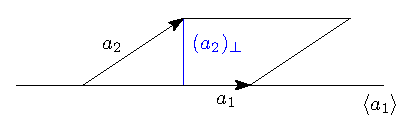
\includegraphics[width=0.4\textwidth]{7_4.eps}
		\label{7_4}
		\caption{Объем параллелепипеда $P(a_1,a_2)$.}
		\label{fig:Задание объема параллелепипеда}
	\end{figure}
	\item $n = 3 \Rightarrow V_3(P(a_1,a_2,a_3)) = V_2(P(a_1,a_2)){\cdot}d(a_3, \langle a_1, a_2 \rangle)$, то есть произведение площади основания на высоту;
	\item[\vdots]
	\item[(n)] По индукции, пусть определено $V_{n-1}(P(a_1, \dotsc, a_{n-1}))$, тогда:
	$$
		V_n(P(a_1,\dotsc,a_n)) =V_{n-1}(P(a_1, \dotsc, a_{n-1})){\cdot}d(a_n,\langle a_1, \dotsc, a_{n-1}\rangle)
	$$
\end{enumerate}
Пока это не очень хорошее определение, поскольку не ясно, зависит ли таким образом заданный объем от порядка $a_1, \dotsc, a_n$. Рассмотрим следующую теорему.
\begin{theorem}
	$V_n(P(a_1,\dotsc, a_n))^2 = \det{(G(a_1,\dotsc,a_n))}$.
\end{theorem}
\begin{proof}
	Докажем по индукции:
	
	\uline{\textbf{База}}: $n = 1 \Rightarrow |a_1|^2 = (a_1,a_1) \Rightarrow$ утверждение верно.
	
	\uline{\textbf{Шаг}}: пусть теорема верна для $n-1 \Rightarrow$ выполним шаг индукции и рассмотрим матрицу Грама $n$-го порядка:
	$$
		G = G(a_1, \dotsc, a_n) = 
		\begin{pmatrix}
			(a_1,a_1) & \dotsc & (a_1, a_{n-1}) & (a_1, a_n) \\
			\vdots & \ddots & \vdots & \vdots \\
			(a_{n-1}, a_1) & \dotsc & (a_{n-1}, a_{n-1}) & (a_{n-1}, a_n) \\ 
			(a_n, a_1) & \dotsc & (a_{n}, a_{n-1}) & (a_n, a_n)
		\end{pmatrix}
	$$
	Запишем вектор $a_n$ в виде суммы ортогональной проекции и ортогональной составляющей:
	$$
		a_n = a_{\|} + a_{\bot} = \lambda_1 a_1 + \dotsc + \lambda_{n-1} a_{n-1} + a_\bot
	$$
	Подставим его в матрицу и рассмотрим изменения в последнем столбце. Поскольку $(a_i, a_\bot) = 0, \, \forall i < n$, то получим следующее:
	$$
		(a_i, a_n) = (a_i,  \lambda_1 a_1 + \dotsc + \lambda_{n-1} a_{n-1} + a_\bot) = \lambda_1 (a_i, a_1) + \dotsc + \lambda_{n-1}(a_i, a_{n-1}) + (a_i, a_\bot)
	$$
	$$
		\begin{pmatrix}
			(a_1, a_n)\\
			\vdots \\
			(a_{n-1}, a_n)\\
			(a_n, a_n)
		\end{pmatrix} =
		\begin{pmatrix}
			\lambda_1 (a_1, a_1) &+& \dotsc &+& \lambda_{n-1}(a_1, a_{n-1}) &+& 0 \\
			\vdots & \vdots & \vdots & \vdots & \vdots & \vdots & \vdots  \\
			\lambda_1 (a_{n-1}, a_1) &+& \dotsc &+& \lambda_{n-1}(a_{n-1}, a_{n-1}) &+& 0 \\
			\lambda_1 (a_n, a_1) &+& \dotsc &+& \lambda_{n-1}(a_n, a_{n-1}) &+& (a_n, a_\bot)
		\end{pmatrix} =
	$$
	$$
		= \lambda_1{\cdot}
		\begin{pmatrix}
			(a_1, a_1)\\
			\vdots\\
			(a_{n-1},a_1)\\
			(a_n, a_n)
		\end{pmatrix} + \dotsc + \lambda_{n-1}{\cdot}
		\begin{pmatrix}
			(a_1, a_{n-1})\\
			\vdots\\
			(a_{n-1},a_{n-1})\\
			(a_n, a_{n-1})
		\end{pmatrix} + 
		\begin{pmatrix}
			0 \\
			\vdots\\
			0 \\
			(a_n, a_\bot)
		\end{pmatrix}
	$$
	таким образом, получили линейную комбинацию от $1$-го до $n-1$-го столбца плюс еще один столбец. По свойству определителей выполнено следующее:
	$$
		\begin{vmatrix}
			x_1 & \dotsc & x_{n-1} & \lambda_1 x_1 + \dotsc + \lambda_{n-1} x_{n-1} + x_n
		\end{vmatrix} = 
		\begin{vmatrix}
			x_1 & \dotsc & x_{n-1} & \lambda_1 x_1 
		\end{vmatrix} + \dotsc + 
		\begin{vmatrix}
			x_1 & \dotsc & x_{n-1} & \lambda_{n-1} x_{n-1} 
		\end{vmatrix} + 
	$$	
	$$
		+
		\begin{vmatrix}
			x_1 & \dotsc & x_{n-1} & x_n
		\end{vmatrix} = 0 + \dotsc + 0 + 
		\begin{vmatrix}
			x_1 & \dotsc & x_{n-1} & x_n
		\end{vmatrix} = 
		\begin{vmatrix}
			x_1 & \dotsc & x_{n-1} & x_n
		\end{vmatrix}
	$$
	Поскольку $a_n = a_{\|} + a_{\bot}$, то $(a_n, a_\bot) = (a_{\|} + a_\bot, a_\bot) = |a_\bot|^2$. Рассмотрим определитель матрицы Грама:
	$$
		|G| = |G(a_1, \dotsc, a_n)| = 
		\begin{vmatrix}
			(a_1,a_1) & \dotsc & (a_1, a_{n-1}) & 0 \\
			\vdots & \ddots & \vdots & \vdots \\
			(a_{n-1},a_1) & \dotsc & (a_{n-1}, a_{n-1}) & 0\\
			(a_n, a_1) & \dotsc & (a_n, a_{n-1}) & |a_\bot|^2
		\end{vmatrix} = |a_\bot|^2{\cdot}|G(a_1, \dotsc, a_{n-1})|
	$$
	где $|a_\bot|^2 = d(a_n, \langle a_1, \dotsc, a_{n-1}\rangle)^2$ верно по определению, тогда: 
	$$
		|G(a_1,\dotsc, a_n)| = |G(a_1,\dotsc, a_{n-1})|{\cdot}d(a_n, \langle a_1, \dotsc, a_{n-1}\rangle)^2
	$$
	что дает равенство определителя матрицы Грама квадрату объема параллелепипеда.
\end{proof}
\begin{corollary}
	Определитель матрицы Грама неотрицателен: $\det{G} \geq 0, \, \forall a_1, \dotsc, a_n$.
\end{corollary}
\begin{proof}
	Доказательство по теореме выше.
\end{proof}
\begin{corollary}
	$|G(a_1, \dotsc, a_n)| = 0 \Leftrightarrow a_1, \dotsc, a_n$ - линейно зависимы.
\end{corollary}
\begin{proof}\hfill\\
	$(\Leftarrow)$ Пусть $a_n = \lambda_1 a_1 + \dotsc + \lambda_{n-1} a_{n-1}$, тогда будет верно:
	$$
		\begin{vmatrix}
			(a_1,a_1) & \dotsc & (a_1, a_{n-1}) & (a_1, \lambda_1 a_1 + \dotsc + \lambda_{n-1} a_{n-1}) \\
			\vdots & \ddots & \vdots & \vdots \\
			(a_n,a_1) & \dotsc & (a_n, a_{n-1}) & (a_n, \lambda_1 a_1 + \dotsc + \lambda_{n-1} a_{n-1})
		\end{vmatrix} = 0
	$$
	
	$(\Rightarrow)$ $|G(a_1)|, \, |G(a_1,a_2)|, \dotsc, |G(a_1, \dotsc, a_k)|, \, |G(a_1, \dotsc, a_k, a_{k+1})|, \dotsc, |G(a_1, \dotsc, a_n)| = 0 \Rightarrow$ если все равны нулю, то $G(a_1) = |a_1|^2 = 0 \Rightarrow a_1 = 0 \Rightarrow$ вектора линейно зависимы. 
	
	В том случае, если начиная с некоторого номера $k, \, |G(a_1, \dotsc, a_k)| \neq 0$, но $|G(a_1, \dotsc, a_k, a_{k+1})| = 0$, тогда:
	$$
 		V_k(P(a_1, \dotsc, a_k)) \neq 0, \, V_{k+1}(P(a_1, \dotsc, a_{k+1})) = 0 \Rightarrow
	$$	
	$$	
		\Rightarrow V_{k+1}(P(a_1, \dotsc, a_{k+1})) = V_k(P(a_1,\dotsc, a_k)){\cdot}d(a_{k+1},\langle a_1, \dotsc, a_k \rangle) = 0 \Rightarrow d(a_{k+1}, \langle a_1, \dotsc, a_k \rangle) = 0 \Rightarrow
	$$
	$$
		\Rightarrow a_{k+1} = (a_{k+1})_{\|} + (a_{k+1})_{\bot} = (a_{k+1})_{\|}
	$$
	где последнее верно поскольку $|(a_{k+1})_\bot| = d(a_{k+1},\langle a_1, \dotsc, a_k \rangle ) = 0 \Rightarrow a_{k+1} = (a_{k+1})_{\|} \in \langle a_1, \dotsc, a_k \rangle \Rightarrow$ получили линейную зависимость векторов $a_1, \dotsc, a_n$.
\end{proof}

\begin{corollary}
	При перестановке векторов $a_1, \dotsc, a_n$ матрица Грама не меняется $\Rightarrow$ объем не зависит от порядка $a_1, \dotsc, a_n$.
\end{corollary}

Пусть $e_1, \dotsc, e_n, \tilde{e}_1, \dotsc, \tilde{e}_n$ - два базиса, $C$ - матрица перехода, $G = G(e_1,\dotsc, e_n), \, \widetilde{G} = G(\tilde{e}_1, \dotsc, \tilde{e}_n)$. Обозначим следующим образом элементы этих матриц: $g_{ij} = (e_i,e_j), \, \tilde{g}_{ij} = (\tilde{e}_i, \tilde{e}_j) \colon \tilde{e}_i = c_i^j e_j$ (суммирование по индексу $j$). 

Пусть $\tilde{e}_i = c_i^k e_k, \, \tilde{e}_j = c_j^l e_l \Rightarrow$ подставим и получим следующее:
$$
	\tilde{g}_{ij} = (c_i^k e_k, c_j^l e_l) = 
	\begin{cases}
		c_i^k c_j^l{\cdot} g_{kl}, & \MK = \MR \\[5pt]
		\overline{c_i^k}c_j^l{\cdot} g_{kl}, & \MK = \MC
	\end{cases}
$$
или в матричном виде для случая $\MK = \MR$ получим такой результат:
$$
	\widetilde{G} =
	\begin{pmatrix}
		c_1^1 & \dotsc & c_1^n \\
		\vdots & \ddots & \vdots \\
		c_n^1 & \dotsc & c_n^n 
	\end{pmatrix}{\cdot}
	\begin{pmatrix}
		g_{11} & \dotsc & g_{1n} \\
		\vdots & \ddots & \vdots \\
		g_{n1} & \dotsc & g_{nn} 
	\end{pmatrix}{\cdot}
	\begin{pmatrix}
		c_1^1 & \dotsc & c_n^1 \\
		\vdots & \ddots & \vdots \\
		c_1^n & \dotsc & c_n^n 
	\end{pmatrix} = C^T G C
$$
\begin{corollary}
	Пусть $G$ - матрица Грама над $\MR$ для некоторого базиса, тогда существует невырожденная матрица $C \colon G = C^T C$.
\end{corollary}
\begin{proof}
	Возьмем первый базис произвольный, а второй ортонормированный, тогда:
	$$
		G_1 = E, \, G = G_2 = C^T G_1 C = C^T E C = C^T C
	$$
\end{proof}
\newpage
\section*{Метод наименьших квадратов}
Рассмотрим следующую систему уравнений:
$$
	\left\{
		\begin{matrix}
			a_1^1 x_1 + \dotsc + a_1^n x_n & = & b_1 \\
			\ddots & \vdots & \vdots \\
			a_m^1 x_1 + \dotsc + a_m^n x_n & = & b_m
		\end{matrix}
	\right., \, m > n
$$
Поскольку $m > n$, то скорее всего решений нет. Данная система эквивалентна следующей:
$$
	a_1 x_1 + \dotsc + a_n x_n = b, \, a_1 = 
	\begin{pmatrix}
		a_1^1 \\
		\vdots \\
		a_m^1
	\end{pmatrix}, \dotsc, a_n = 
	\begin{pmatrix}
		a_1^n \\
		\vdots \\
		a_m^n
	\end{pmatrix}, \, b = 
	\begin{pmatrix}
		b_1 \\
		\vdots \\
		b_m
	\end{pmatrix}	
$$
Пусть $L = \langle a_1 ,\dotsc, a_n \rangle$. Будет ли $b$ принадлежать $L$? Может не принадлежать.
\begin{figure}[H]
	\centering
	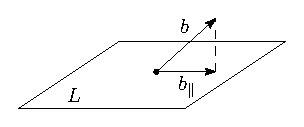
\includegraphics[width=0.3\textwidth]{7_5.eps}
	\label{7_5}
	\caption{Проекция вектора $b$ на $L$.}
	\label{fig:Проекция вектора $b$ на $L$}
\end{figure}
\begin{defn}
	\uwave{Псевдорешением} называется набор $(x_1^\circ, \dotsc x_n^\circ)$, который является решением системы: 
	$$
		a_1 x_1 + \dotsc + a_n x_n = b_{\|}
	$$
\end{defn}
\begin{lemma}Верны следующие утверждения
	\begin{enumerate}[label ={(\arabic*)}]
		\item Псевдорешения всегда существуют; 
		\item Если $a_1, \dotsc, a_n$ линейно независимы, то псевдорешение единственно;
	\end{enumerate}
\end{lemma}
\begin{proof}
	Очевидно, поскольку $a_1 x_1 + \dotsc + a_n x_n$ - произвольный вектор в $L$.
\end{proof}

\begin{corollary}
	$|a_1 x_1 + \dotsc + a_n x_n - b| \geq |a_1 x_1^\circ + \dotsc + a_n x_n^\circ - b| = |b_{\|} - b|$, где $x_1^\circ, \dotsc, x_n^\circ$ - псевдорешение.
\end{corollary}
\begin{rem}
	Другими словами, минимум $|a_1 x_1 + \dotsc + a_n x_n - b|$ достигается на псевдорешении.
\end{rem}
\end{document}